\captionsetup{justification=centering,margin=0cm}
\label{cap:atividade8}  % Forma de referenciar o capítulo no comando \ref

%inicio do capitulo
\chapter[Atividade8: Avaliando os candidatos a sucessor do JPEG]{Atividade 8: Avaliando os candidatos a sucessor do JPEG}

Tá, mas e o sucessor do JPEG? Um bom velho de guerra que já está na internet há muitos anos, mas cuja a tecnologia já é defasada. Uma série de outros formatos melhores tecnicamente surgiram, então vamos analisar esses formatos e seus comportamentos.

\paragrafo Primeiramente, vamos comparar o \textit{ratio} de diferentes formatos. A Tabela abaixo traz essa métrica em três formatos diferentes, WEBP, JPEG XL e AVIf. Dentre eles, o AVIF foi o que teve melhor taxa de compressão, no entanto sua compressão é bem mais pesada que os demais. Ele demorou quase uns dois minutos, enquanto o JEPG XL\footnote{Para a Geração Z uma eternidade.} comprimiu em apenas uns 30 segundos. Dentre eles, o JPEG XL pareceu-me o ideal, chegou muito perto da compressão do AVIF com um pouco mais de tempo do que se comparado ao WEBP.

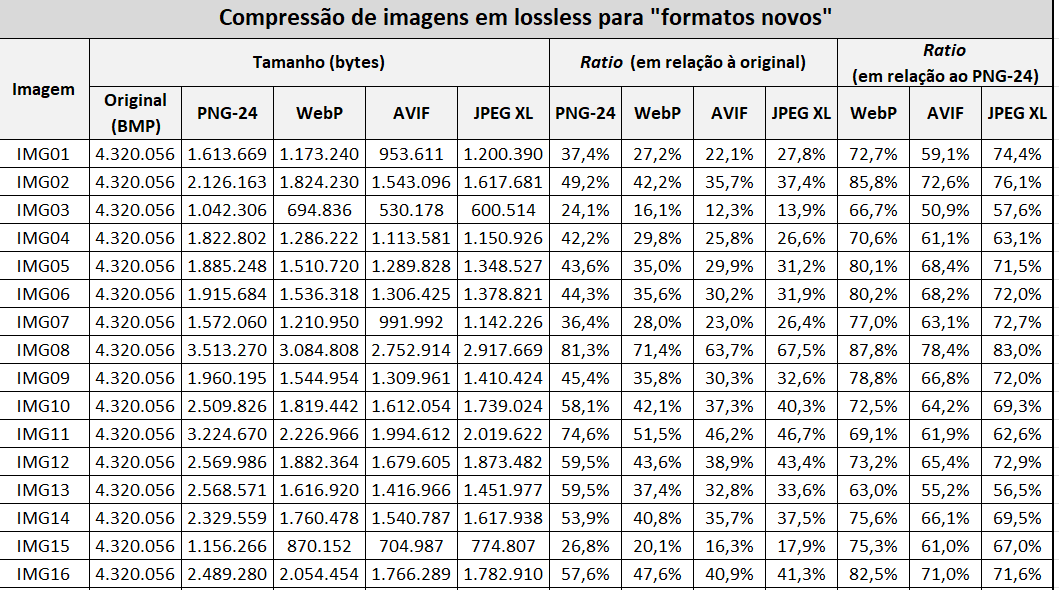
\includegraphics[scale=0.6]{Documeto/1-ElementosTextuais/1-Desenvolvimento/2.png}

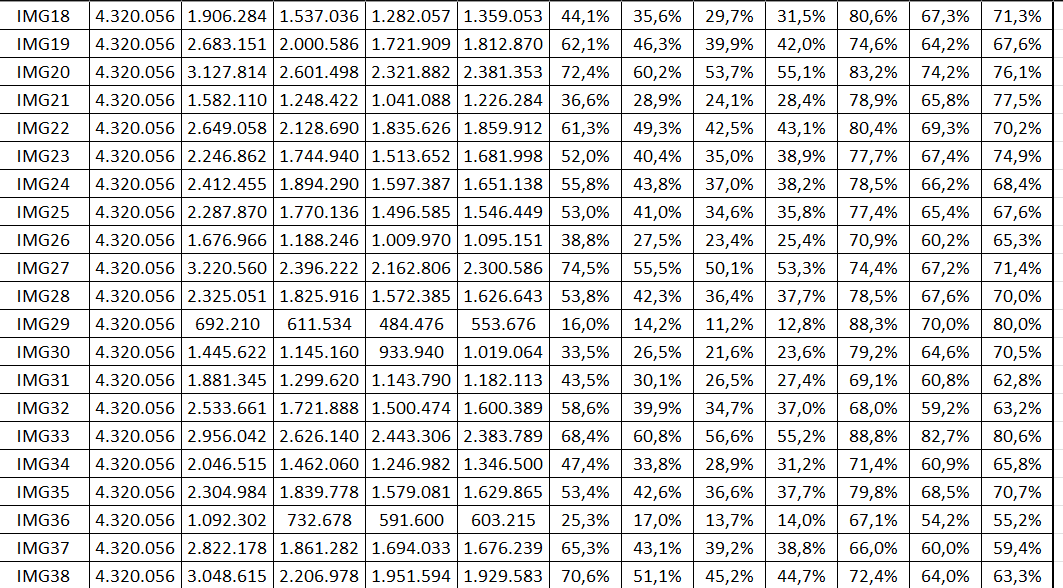
\includegraphics[scale=0.6]{Documeto/1-ElementosTextuais/1-Desenvolvimento/3.png}

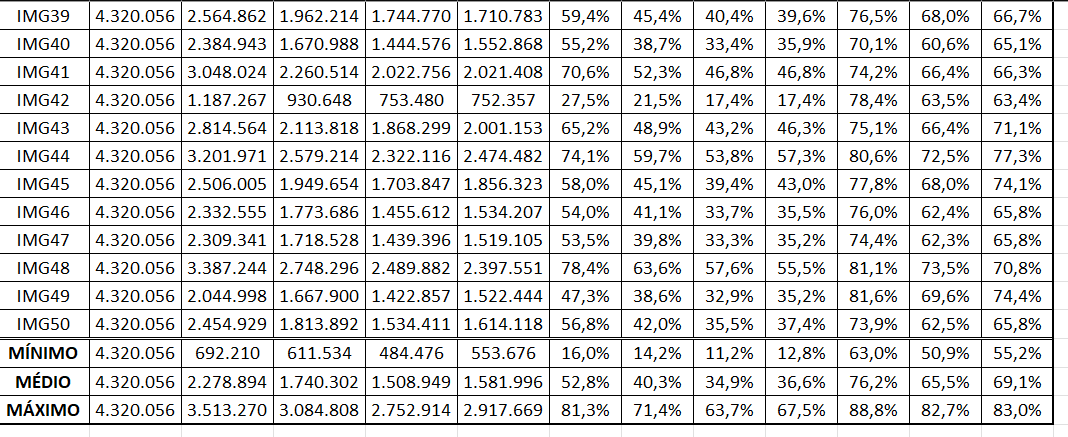
\includegraphics[scale=0.6]{Documeto/1-ElementosTextuais/1-Desenvolvimento/4.png}

\paragrafo  Agora, tem-se a \ref{tab:8b}, que busca comparar diferentes formatos mais hodiernos. Pelas nossas observações, o AVIF acabou por ser o mais indicado se o fator compressão é o mais importante. A sua compressão é muito boa, chegando a resultados surpreendentes; no entanto, seu "peso" acaba por ser muito ruim em alguns momentos. A sua compressão é bastante demorada, não sendo um impeditivo, mas uma desvantagem. Em contra partida, o JPEGXL apresentou taxas de compressão menores, mas bem mais rápidas.

\begin{table}[H]
\centering
\caption{Compressão de imagens em lossy para "formatos novos"
(Qualidade Transparente)}
\label{8b}
\begin{tabularx}{\textwidth}{X|C|C|C|C|C|C|C|C|C}
\hline
 Tamanho (bytes) & ~ & ~ & ~ & ~ & Fator de Qualidade & ~ & ~ & ~ \\ \hline
        IMAGEM & Original (BMP) & JPEG & WebP & HEIC & JPEG XL & JPEG & WebP & HEIC & JPEG XL \\ \hline
        48 & 4.320.056 & 254.090 & 310.686 & 340.733 & 188.416 & 40 & 29 & 42 & 48 \\ \hline
        46 & 4.320.056 & 154.390 & 114.576 & 93.146 & 163.148 & 55 & 45 & 40 & 61 \\ \hline
        39 & 4.320.056 & 202.000 & 183.898 & 781.926 & 104.703 & 55 & 37 & 46 & 65 \\ \hline
        35 & 4.320.056 & 153.780 & 107.850 & 331.787 & 158.098 & 55 & 43 & 60 & 64 \\ \hline
        33 & 4.320.056 & 205.860 & 282.516 & 686.707 & 98.730 & 45 & 68 & 50 & 51 \\ \hline
        18 & 4.320.056 & 94.980 & ~ & 87.412 & 131.860 & 50 & 40 & 45 & 58 \\ \hline
        16 & 4.320.056 & 129.520 & 170.688 & 240.063 & 105.527 & 40 & 70 & 50 & 49 \\ \hline
        3 & 4.320.056 & 54.190 & 27.110 & 79.968 & 43.527 & 75 & 67 & 57 & 82 \\ \hline
\end{tabularx}

\autoriaPropria
\end{table}

\begin{table}[H]
\centering
\caption{Compressão de imagens em lossy para "formatos novos"
(Qualidade "Aceitável")}
\label{8b2}
\begin{tabularx}{\textwidth}{X|C|C|C|C|C|C|C|C|C}
\hline
  Imagem & Tamanho (bytes) & ~ & ~ & ~ & ~ & Fator de Qualidade & ~ & ~ & ~ \\ \hline
        ~ & Original (BMP) & JPEG & WebP & HEIC & JPEG XL & JPEG & WebP & HEIC & JPEG XL \\ \hline
        48 & 4.320.056 & 62.087 & 263.148 & 220.540 & 163.840 & 32 & 26 & 35 & 42 \\ \hline
        46 & 4.320.056 & 141.308 & 96.096 & 93.146 & 186.571 & 40 & 32 & 23 & 48 \\ \hline
        39 & 4.320.056 & 91.853 & 163.702 & 41.503 & 127.290 & 48 & 39 & 46 & 57 \\ \hline
        35 & 4.320.056 & 169.353 & 93.054 & 309.487 & 185.618 & 42 & 34 & 50 & 49 \\ \hline
        33 & 4.320.056 & 153.123 & 245.042 & 115.453 & 128.095 & 31 & 24 & 36 & 39 \\ \hline
        18 & 4.320.056 & 218.938 & ~ & 23.530 & 108.531 & 35 & 33 & 22 & 45 \\ \hline
        16 & 4.320.056 & 165.918 & 147.526 & 67.360 & 92.678 & 32 & 58 & 27 & 40 \\ \hline
        3 & 4.320.056 & 276.802 & 22.946 & 21.170 & 24.625 & 61 & 53 & 39 & 69 \\ \hline
\end{tabularx}

\autoriaPropria
\end{table}

\begin{table}[H]
\centering
\caption{"Compressão de imagens em lossy para ""formatos novos""
(Qualidade Transparente)"}
\label{8c}
\begin{tabularx}{\textwidth}{X|C|C|C|C|C|C|C|C|C}
\hline
  Imagem & Tamanho (bytes) & ~ & ~ & ~ & ~ & Fator de Qualidade & ~ & ~ & ~ \\ \hline
        ~ & Original (BMP) & JPEG & WebP & HEIC & JPEG XL & JPEG & WebP & HEIC & JPEG XL \\ \hline
        48 & 4.320.056 & 62.087 & 263.148 & 220.540 & 163.840 & 32 & 26 & 35 & 42 \\ \hline
        46 & 4.320.056 & 141.308 & 96.096 & 93.146 & 186.571 & 40 & 32 & 23 & 48 \\ \hline
        39 & 4.320.056 & 91.853 & 163.702 & 41.503 & 127.290 & 48 & 39 & 46 & 57 \\ \hline
        35 & 4.320.056 & 169.353 & 93.054 & 309.487 & 185.618 & 42 & 34 & 50 & 49 \\ \hline
        33 & 4.320.056 & 153.123 & 245.042 & 115.453 & 128.095 & 31 & 24 & 36 & 39 \\ \hline
        18 & 4.320.056 & 218.938 & ~ & 23.530 & 108.531 & 35 & 33 & 22 & 45 \\ \hline
        16 & 4.320.056 & 165.918 & 147.526 & 67.360 & 92.678 & 32 & 58 & 27 & 40 \\ \hline
        3 & 4.320.056 & 276.802 & 22.946 & 21.170 & 24.625 & 61 & 53 & 39 & 69 \\ \hline
\end{tabularx}

\autoriaPropria
\end{table}

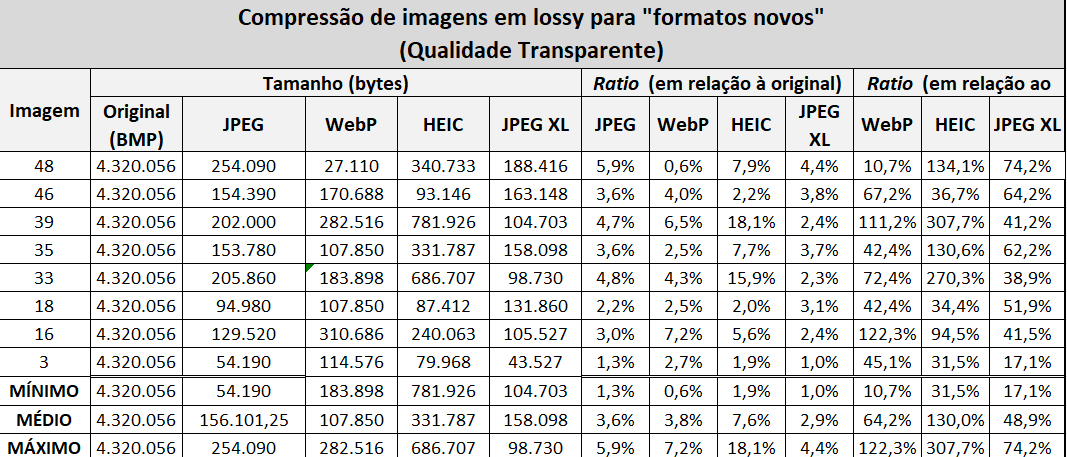
\includegraphics[scale=0.6]{Documeto/1-ElementosTextuais/1-Desenvolvimento/0.png}


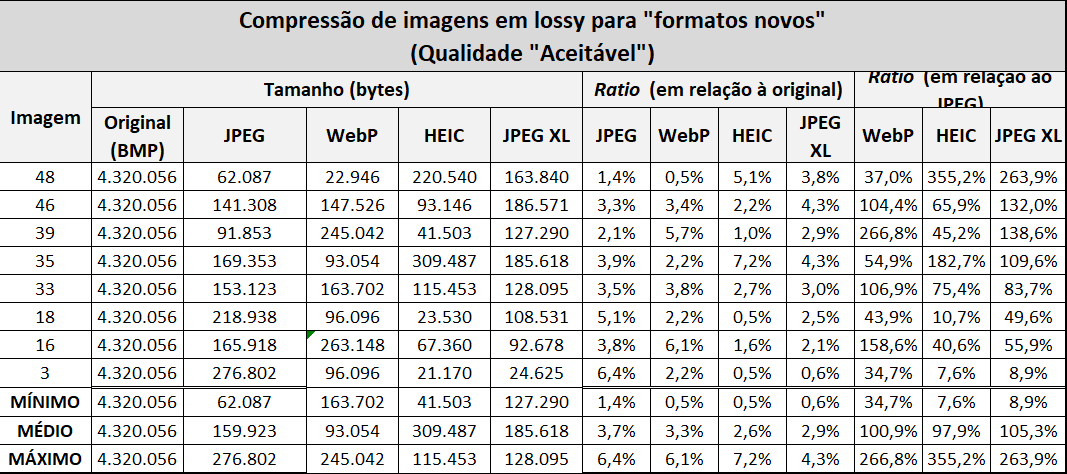
\includegraphics[scale=0.6]{Documeto/1-ElementosTextuais/1-Desenvolvimento/1.png}